\documentclass{beamer}

% --- Escolha de Tema e Cores ---
\usetheme{Madrid}
\usecolortheme{default}

% --- Pacotes e Configurações ---
\usepackage[utf8]{inputenc}
\usepackage{graphicx}
\usepackage{svg} % Pacote para incluir SVG
\usepackage{amsmath}
\usepackage{listings} % Para blocos de código
\usepackage{xcolor} % Para cores no código

% Configuração para blocos de código que já temos no artigo
\definecolor{codegreen}{rgb}{0,0.6,0}
\definecolor{codegray}{rgb}{0.5,0.5,0.5}
\definecolor{codepurple}{rgb}{0.58,0,0.82}
\definecolor{backcolour}{rgb}{0.95,0.95,0.92}

\lstdefinestyle{customStyle}{
    backgroundcolor=\color{backcolour},
    commentstyle=\color{codegreen},
    keywordstyle=\color{magenta},
    numberstyle=\tiny\color{codegray},
    stringstyle=\color{codepurple},
    basicstyle=\ttfamily\footnotesize,
    breakatwhitespace=false,
    breaklines=true,
    captionpos=b,
    keepspaces=true,
    numbers=left,
    numbersep=5pt,
    showspaces=false,
    showstringspaces=false,
    showtabs=false,
    tabsize=2
}
\lstset{style=customStyle}


% --- Informações do Título ---
\title[Análise de Dependências Go]{Gestão de Dependências em Projetos Go com Ordenação Topológica}
\author{Nicholas Pereira Cristófaro \and Marcos Campos Dias}
\institute{Pontifícia Universidade Católica de Minas Gerais (PUC Minas)}
\date{Junho de 2025}

% --- Início do Documento ---
\begin{document}

% ---------------------------------------------------------------
% SLIDE 1: Título
% ---------------------------------------------------------------
\begin{frame}
  \titlepage
\end{frame}

% ---------------------------------------------------------------
% SLIDE 2: Sumário
% ---------------------------------------------------------------
\begin{frame}
    \frametitle{Sumário}
    \tableofcontents
\end{frame}

% ---------------------------------------------------------------
\section{Introdução}
% ---------------------------------------------------------------
\begin{frame}
  \frametitle{Introdução: O Problema}
  
  \begin{block}{O Desafio em Software Moderno}
    A gestão da complexa rede de dependências é um desafio central na engenharia de software , por vezes referido como "inferno de dependências".
  \end{block}
  
  \begin{alertblock}{O Caso Específico do Go}
    \itemize{
      \item A linguagem impõe uma ordem de inicialização estrita para pacotes.
      \item As funções \texttt{init()} de um pacote só executam após suas dependências serem inicializadas.
      \item \textbf{Dependências Cíclicas} causam um erro fatal de compilação.
    }
  \end{alertblock}
\end{frame}

\section{Introdução}
% ---------------------------------------------------------------
\begin{frame}
    \begin{figure}
        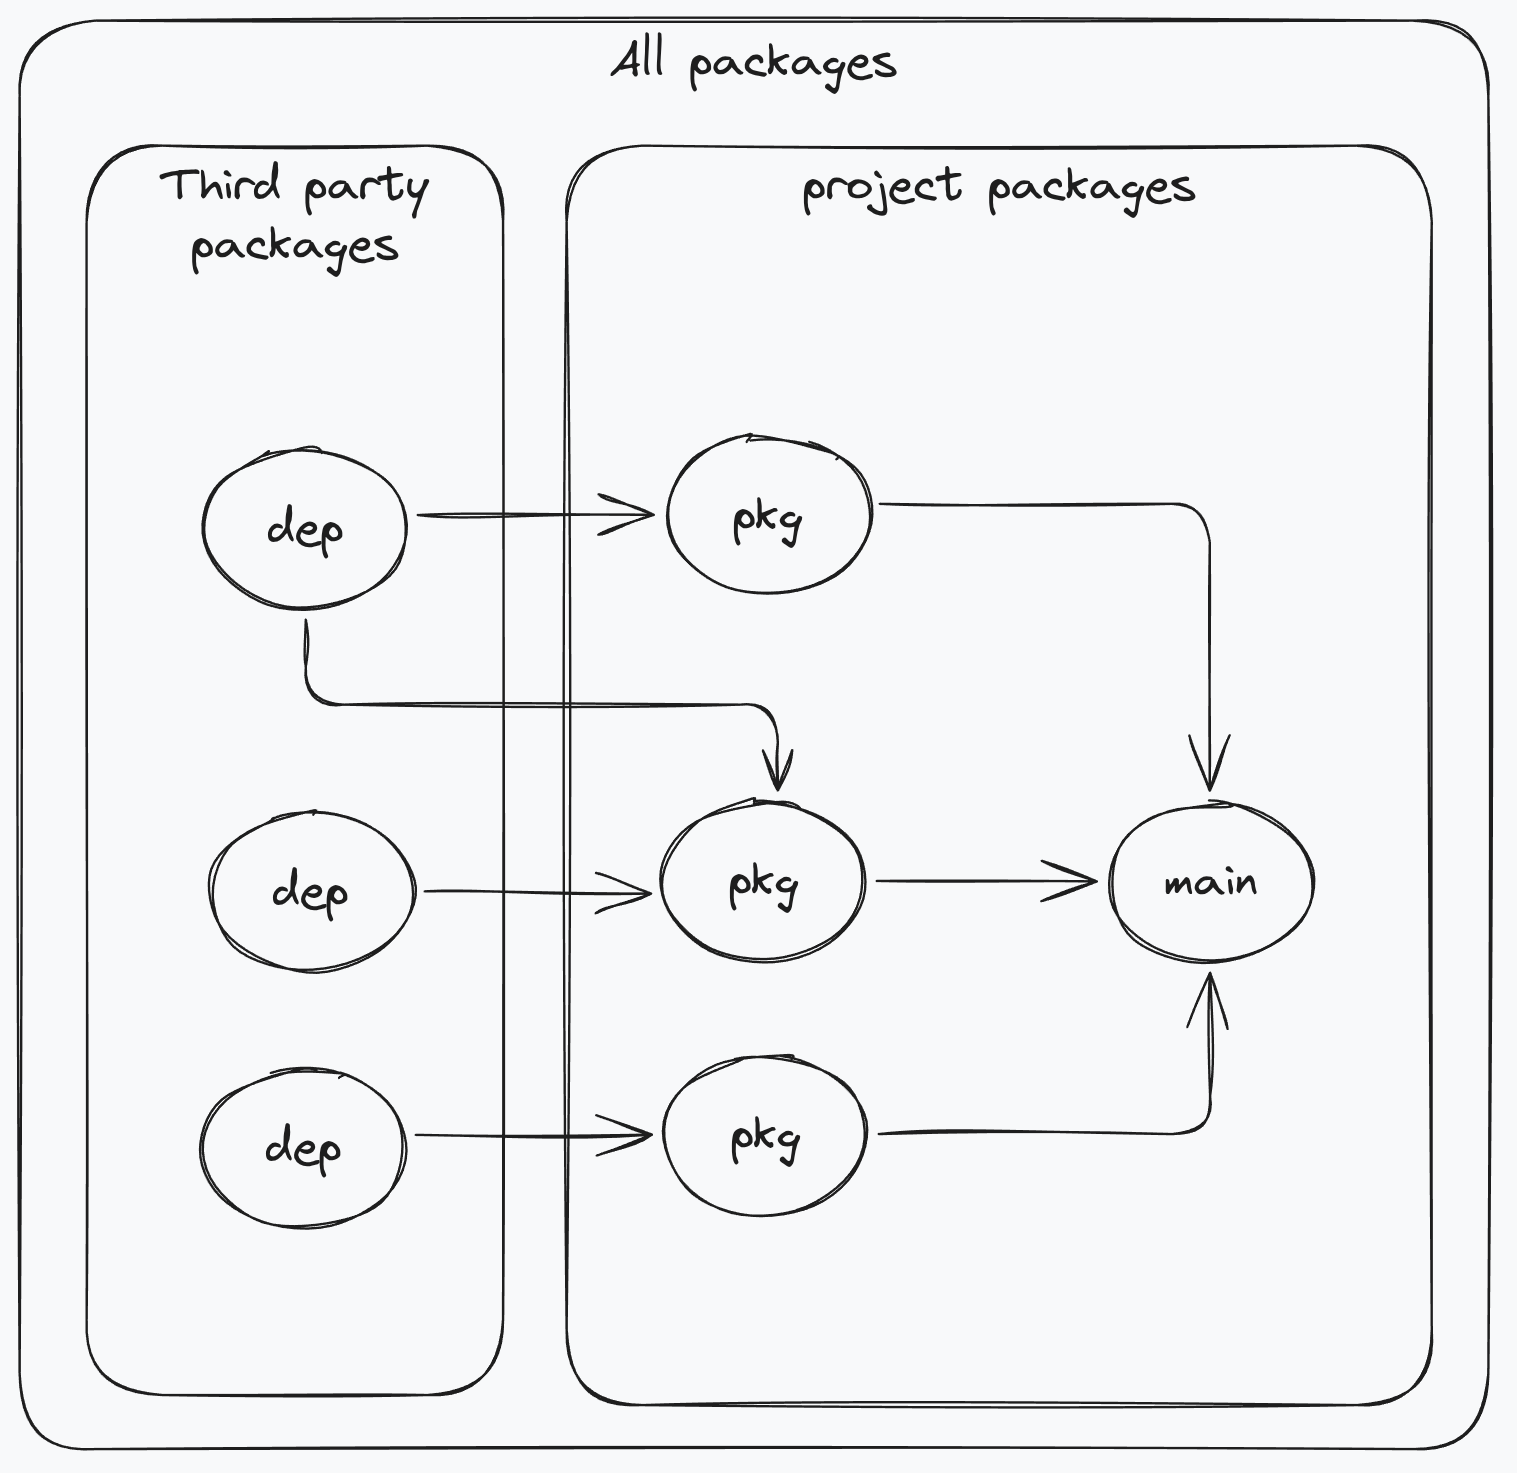
\includegraphics[width=0.6\textwidth]{images/package_overview.png}
        \caption{visualização de um projeto em Golang.}
        \label{fig:grafo-ciclico}
    \end{figure}
\end{frame}


\begin{frame}
    \frametitle{A Solução Proposta}
    
    \begin{itemize}
        \item \textbf{Modelagem:} Representar o projeto e suas dependências como um \textbf{Grafo Direcionado}.
        \begin{itemize}
            \item Pacotes Go $\rightarrow$ Vértices
            \item Imports $\rightarrow$ Arestas
        \end{itemize}
        \bigskip
        \item \textbf{Processamento:} Aplicar a \textbf{Ordenação Topológica} para encontrar a sequência de compilação.
        \bigskip
        \item \textbf{Resultado:} Uma ferramenta em Python que automatiza essa análise e gera uma \textbf{visualização clara} da arquitetura do projeto.
    \end{itemize}
\end{frame}

\begin{frame}
    \begin{figure}
        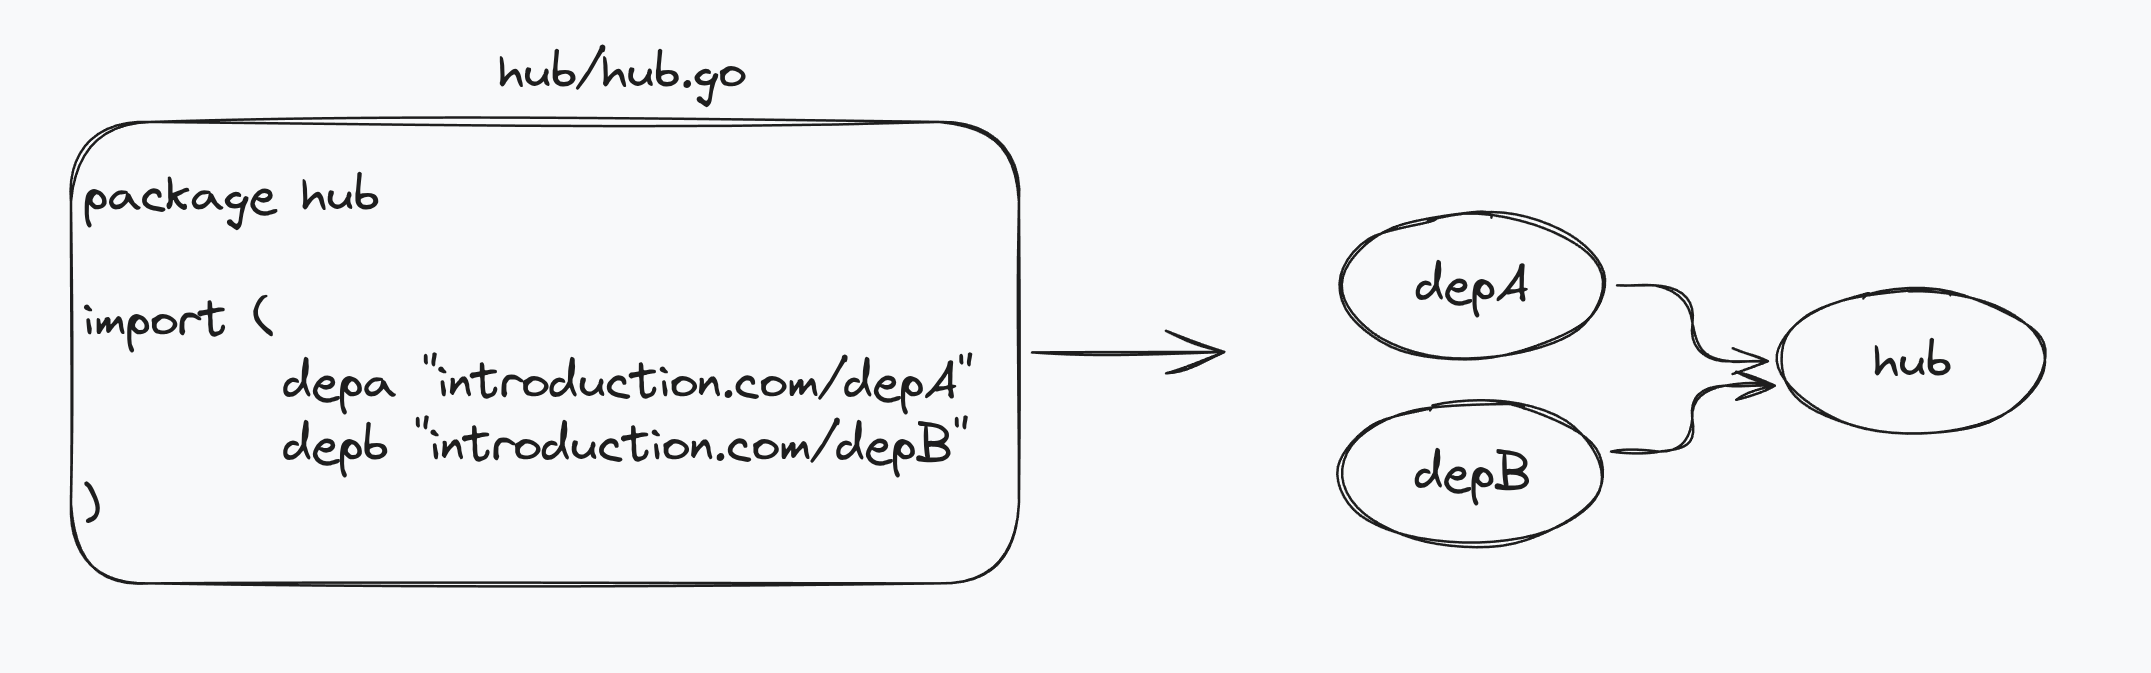
\includegraphics[width=1\textwidth]{images/model.png}
        \caption{representação visual da modelagem.}
        \label{fig:modelagem}
    \end{figure}
\end{frame}

% ---------------------------------------------------------------
\section{Metodologia}
% ---------------------------------------------------------------
\begin{frame}
  \frametitle{Fundamentação: Ordenação Topológica}
  
    \begin{block}{Definição}
        Uma ordenação topológica de um Grafo Acíclico Direcionado (DAG) é uma ordenação linear de seus vértices tal que para toda aresta direcionada $(u, v)$, o vértice $u$ vem antes de $v$ na ordenação.
    \end{block}

    \begin{alertblock}{Pré-requisito: Ausência de Ciclos}
        Se o grafo contiver um ciclo, a ordenação topológica é impossível. A Figura~\ref{fig:grafo-ciclico} ilustra essa condição.
    \end{alertblock}
    
    \begin{figure}
        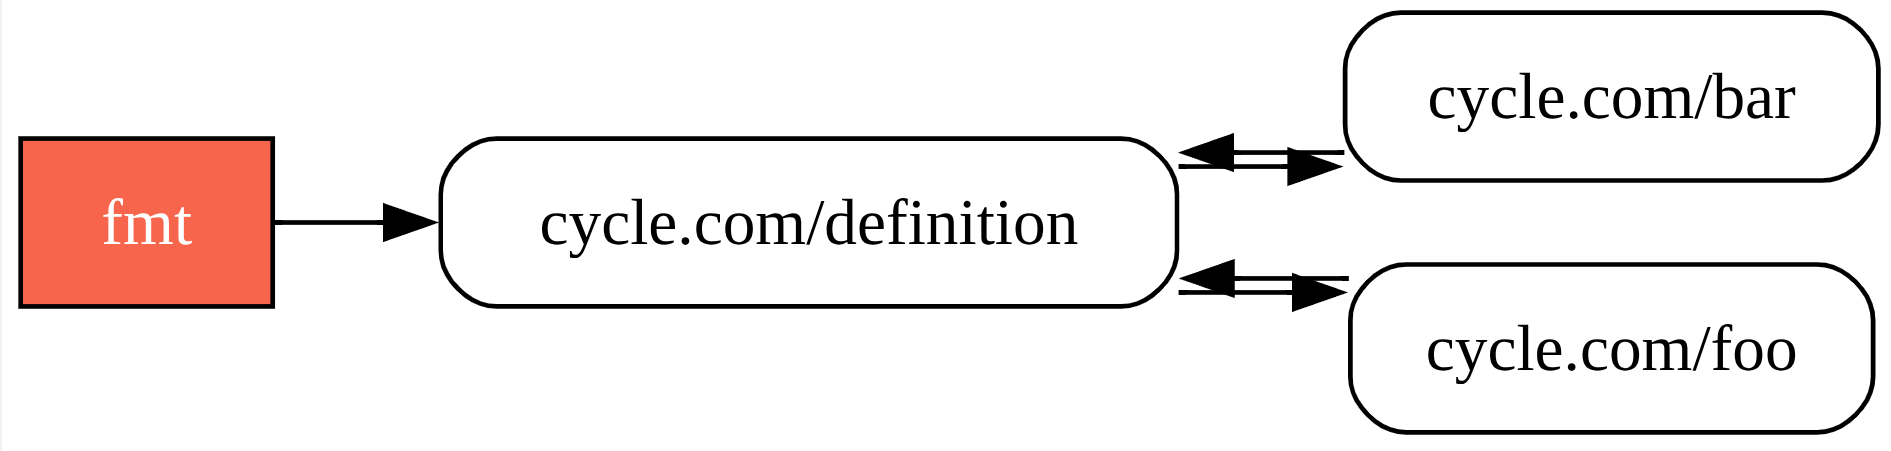
\includegraphics[width=0.6\textwidth]{images/cycle.png}
        \caption{Representação das relações entre pacotes em Golang}
        \label{fig:golang-overview}
    \end{figure}
\end{frame}

% ---------------------------------------------------------------
\begin{frame}[fragile]
    \frametitle{O Algoritmo de Kahn (Pseudocódigo)}
    
    A abordagem escolhida, proposta por Kahn em 1962, funciona de maneira iterativa.
    
    \begin{lstlisting}[language={}, basicstyle=\tiny\ttfamily]
L = Lista vazia que contera os elementos ordenados
S = Conjunto de todos os nos sem arestas de entrada

enquanto S nao esta vazio faca
  remover um no n de S
  adicionar n em L
  
  para cada no m com uma aresta e de n para m faca
    remover aresta e do grafo
    se m nao tem mais arestas de entrada entao
      inserir m em S

se o grafo ainda contem arestas entao
  retornar erro (grafo tem ciclo)
senao
  retornar L (ordenacao)
    \end{lstlisting}
\end{frame}

% ---------------------------------------------------------------
\section{A Ferramenta Desenvolvida}
% ---------------------------------------------------------------
\begin{frame}
  \frametitle{Arquitetura e Fluxo de Execução}

  \begin{figure}
    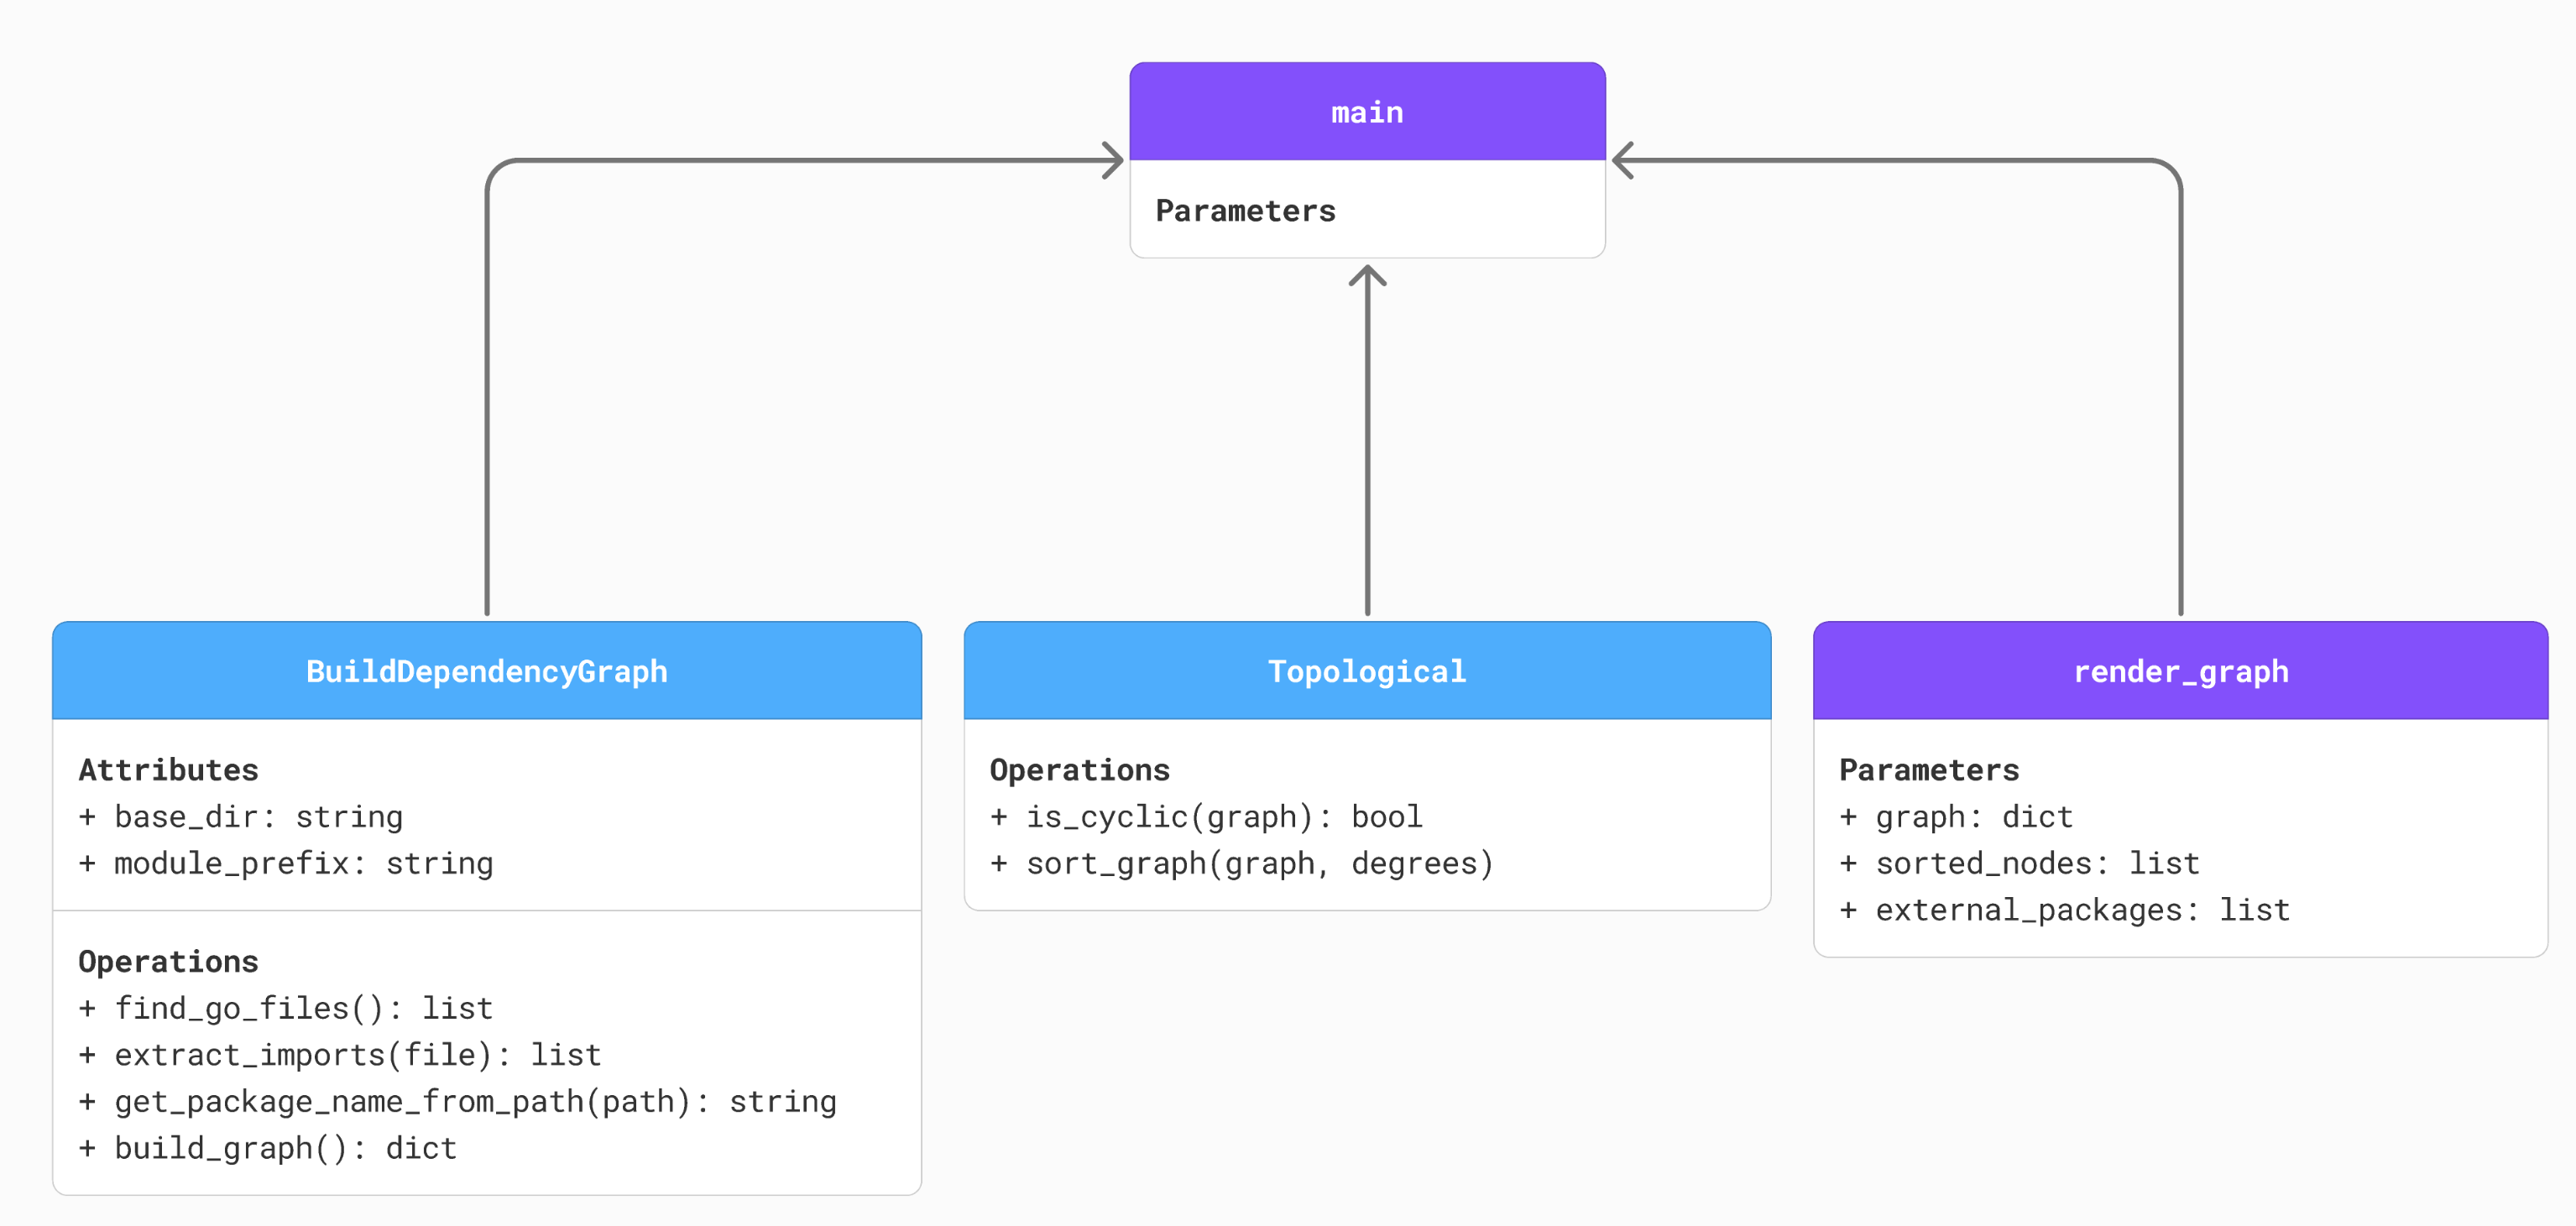
\includegraphics[width=\textwidth]{images/diagrama_classes.png}
    \caption{Fluxo principal: Extração, Processamento e Visualização.}
  \end{figure}
\end{frame}

% ---------------------------------------------------------------
\begin{frame}[fragile]
    \frametitle{Detalhe da Implementação: Extração e Visualização}
    
    \begin{exampleblock}{Extração de Dependências com Regex}
        \begin{lstlisting}[language=Python, basicstyle=\tiny\ttfamily]
# Encontra blocos: import (...)
import_block_match = re.search(r'import\s+\((.*?)\)', ...)
# Encontra linhas unicas: import "..."
single_imports = re.findall(r'import\s+"([^"]+)"', ...)
        \end{lstlisting}
    \end{exampleblock}

    \begin{exampleblock}{Visualização em Camadas com Graphviz}
        \begin{lstlisting}[language=Python, basicstyle=\tiny\ttfamily]
# Agrupa nos em subgrafos para alinhamento em camadas
for layer in sorted_nodes:
    with dot.subgraph() as s:
        s.attr(rank='same') # Forca o mesmo rank (alinhamento)
        for node_name in layer:
            ...
        \end{lstlisting}
    \end{exampleblock}
    A diretiva \texttt{rank='same'} é a chave para o alinhamento visual das camadas.
\end{frame}


% ---------------------------------------------------------------
\section{Resultados: Estudo de Caso}
% ---------------------------------------------------------------
\begin{frame}
  \frametitle{Caso 1: Aplicação Simples}
    \begin{figure}
        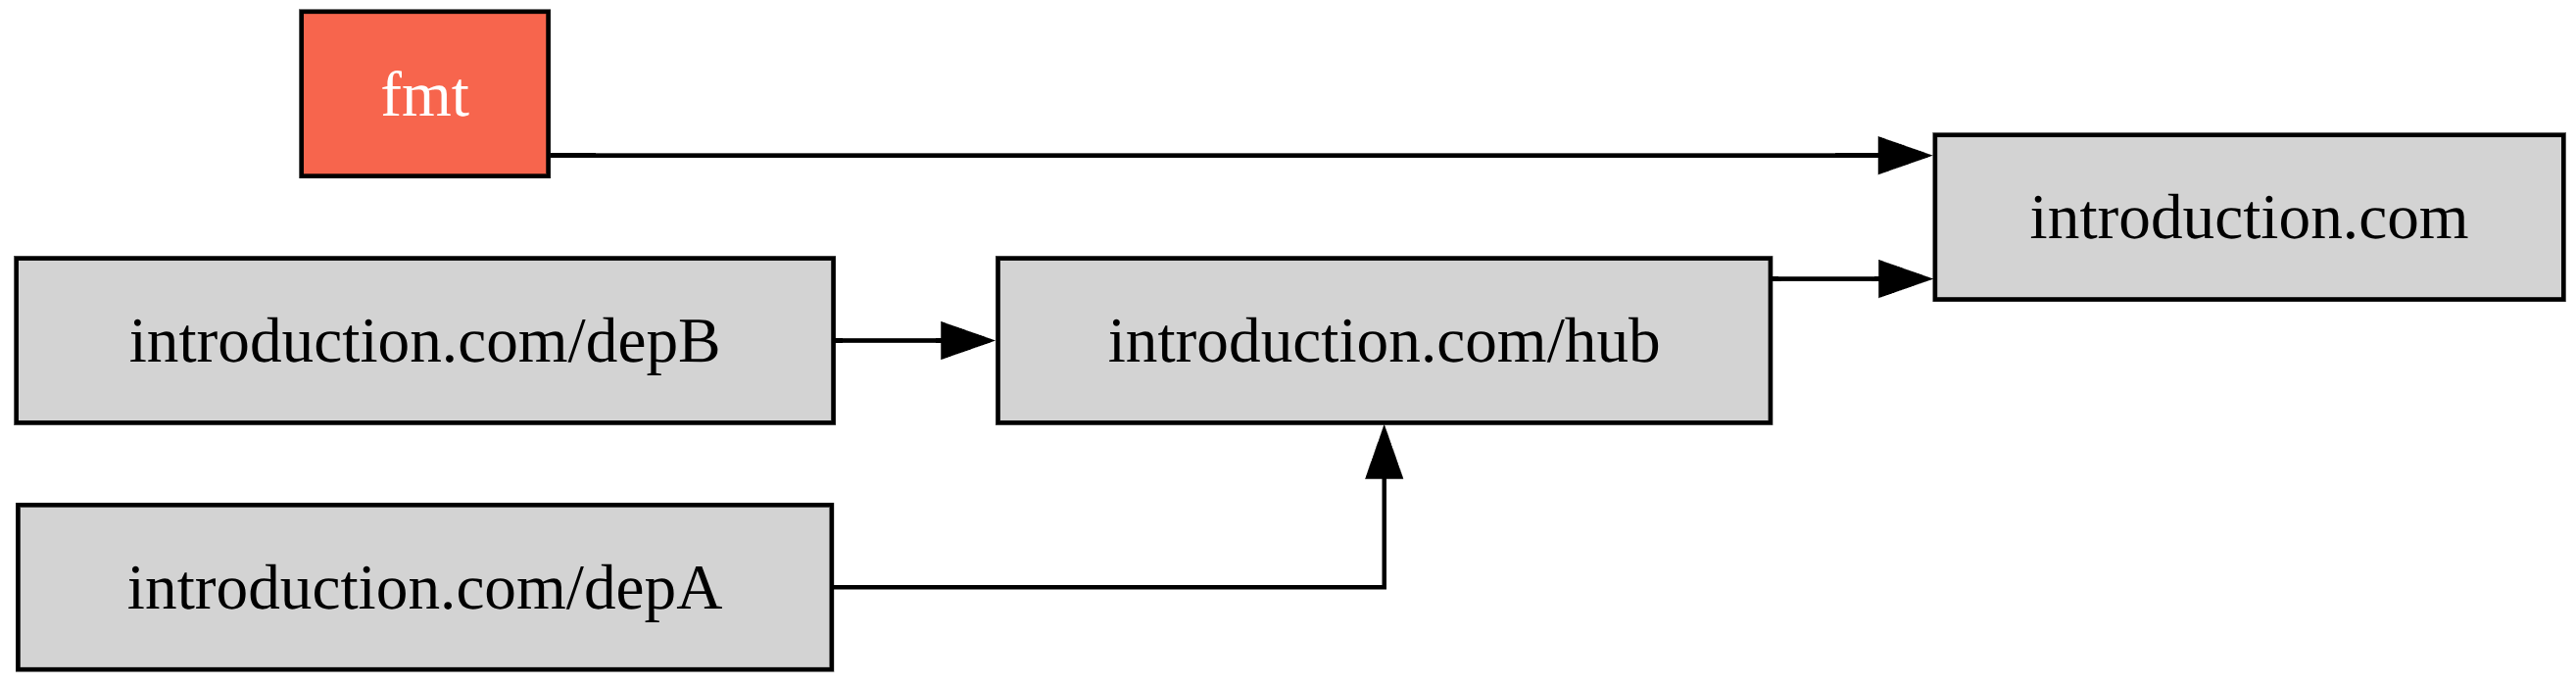
\includegraphics[width=0.9\textwidth]{images/init_example.png}
        \caption{Grafo de um projeto simples com dependências lineares.}
    \end{figure}
    \begin{itemize}
        \item Demonstra uma arquitetura clara, com baixo acoplamento.
        \item As camadas progridem linearmente da esquerda (dependências) para a direita (aplicação).
    \end{itemize}
\end{frame}

\begin{frame}
  \frametitle{Caso 2: Biblioteca de Framework (Cobra)}
    \begin{figure}
        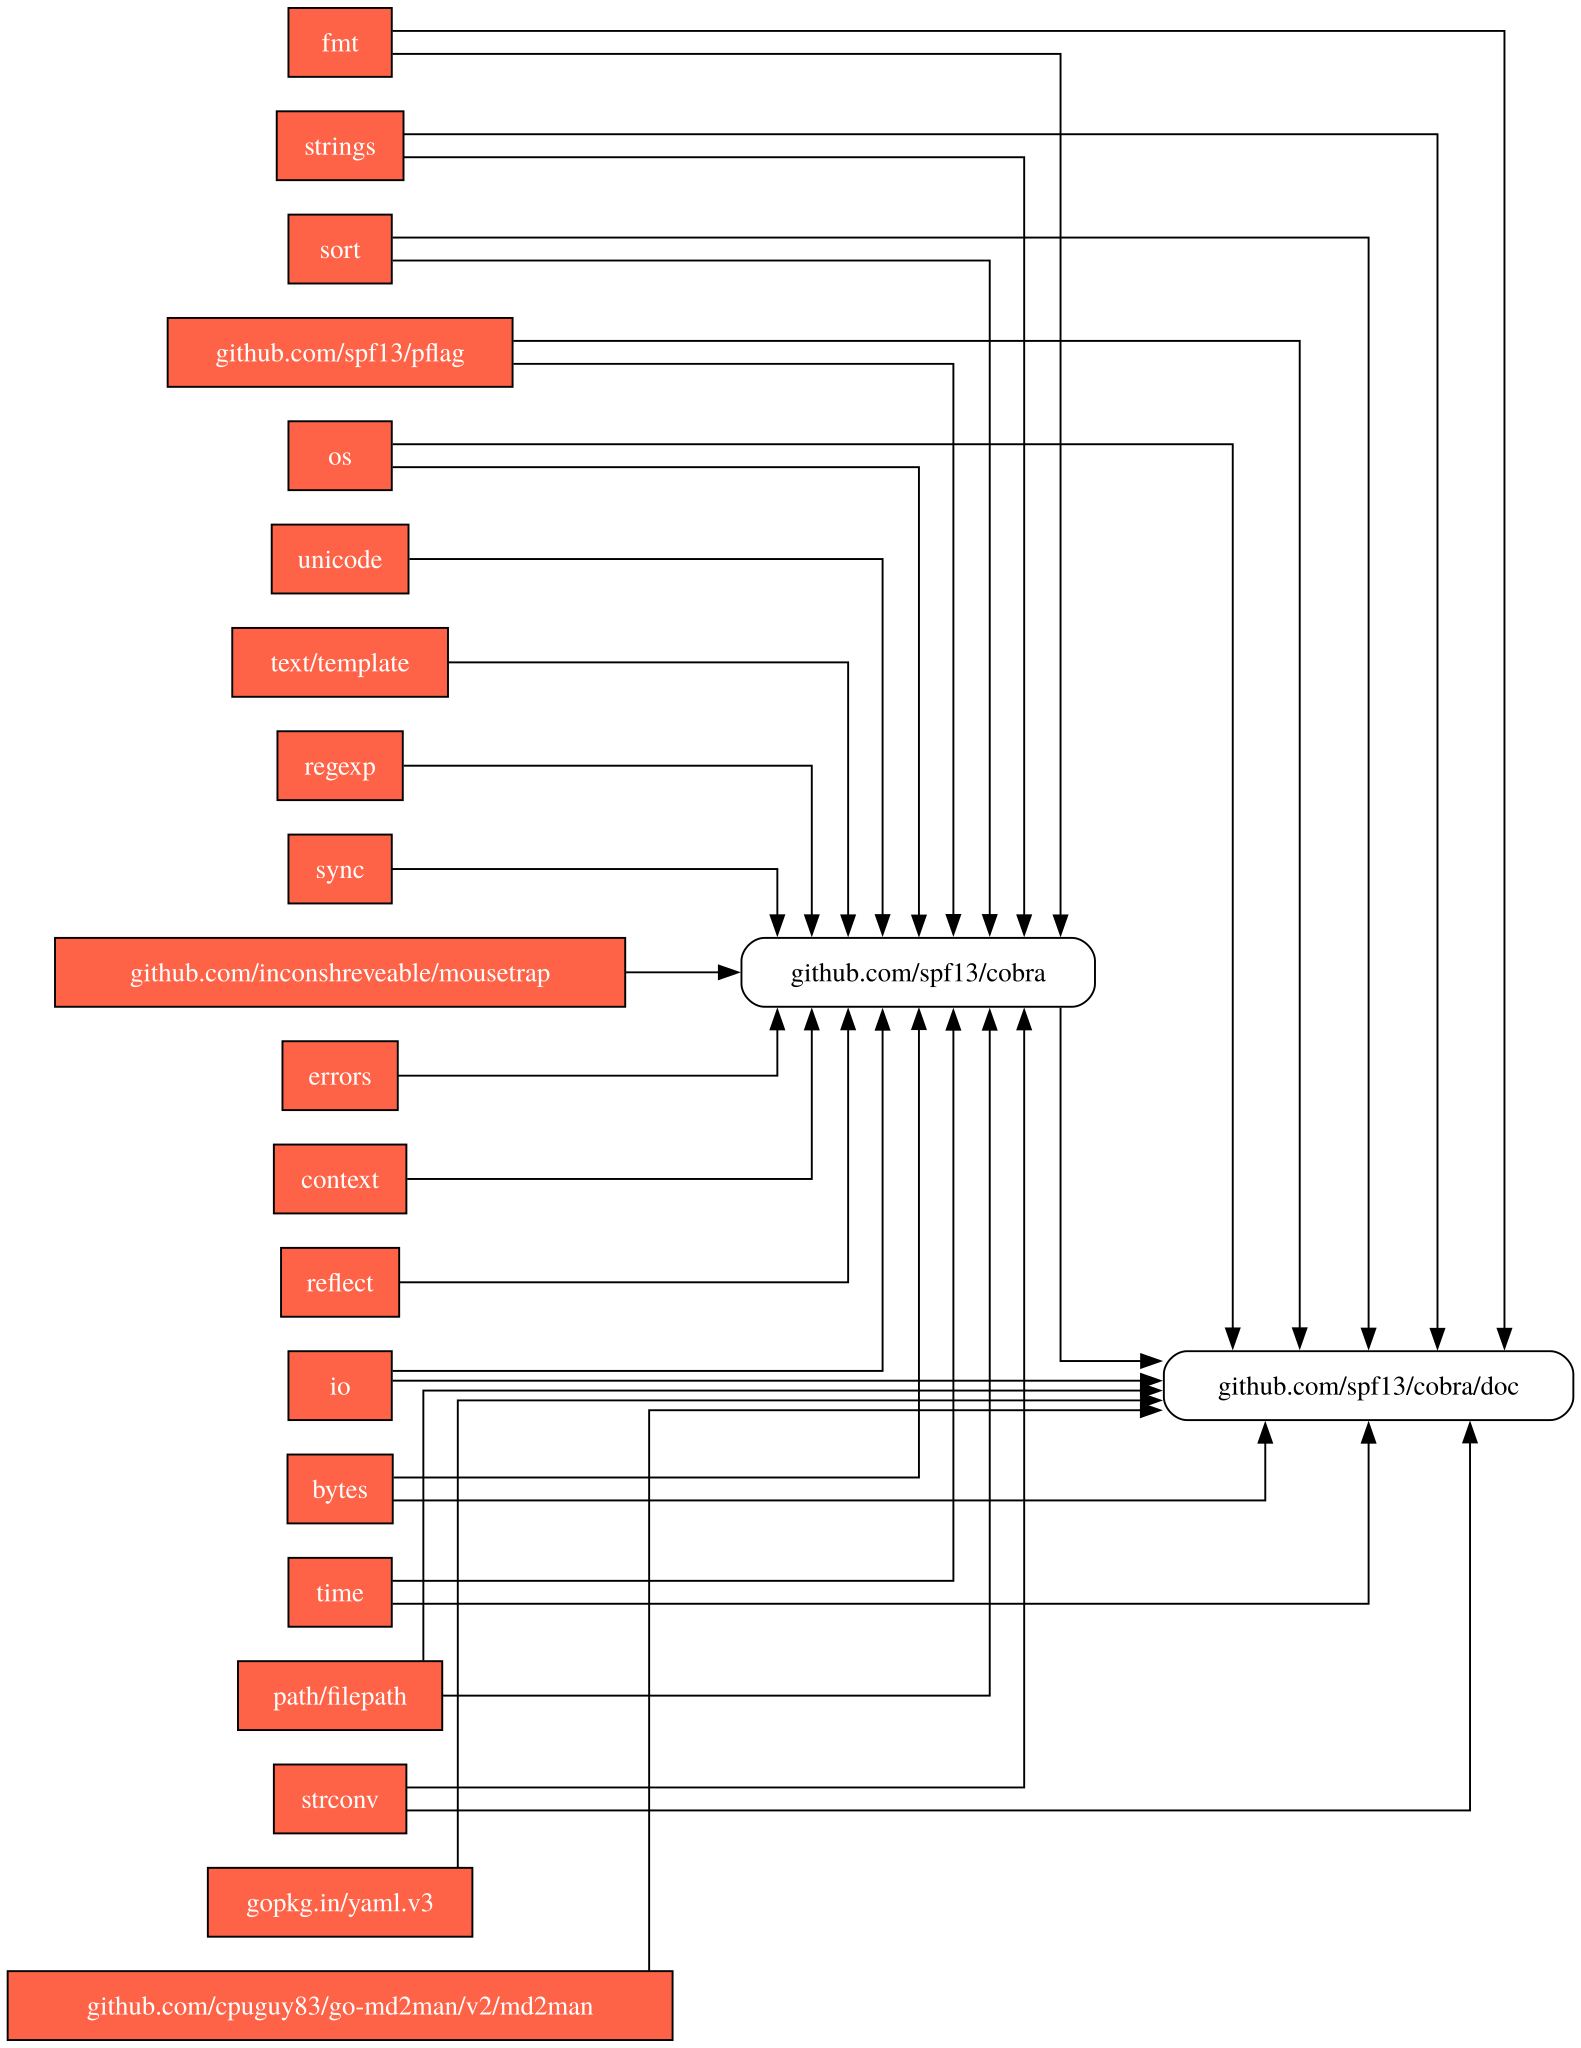
\includegraphics[width=0.5\textwidth]{images/github.com_spf13_cobra.png}
        \caption{Grafo da biblioteca `Cobra`.}
    \end{figure}
    \begin{itemize}
        \item Revela um padrão de "hub-e-spoke".
        \item O pacote central \texttt{cobra} é um "hub" do qual muitos outros dependem, típico de frameworks.
    \end{itemize}
\end{frame}

\begin{frame}
  \frametitle{Caso 3: Bindings para GUI (gotk3)}
    \begin{figure}
        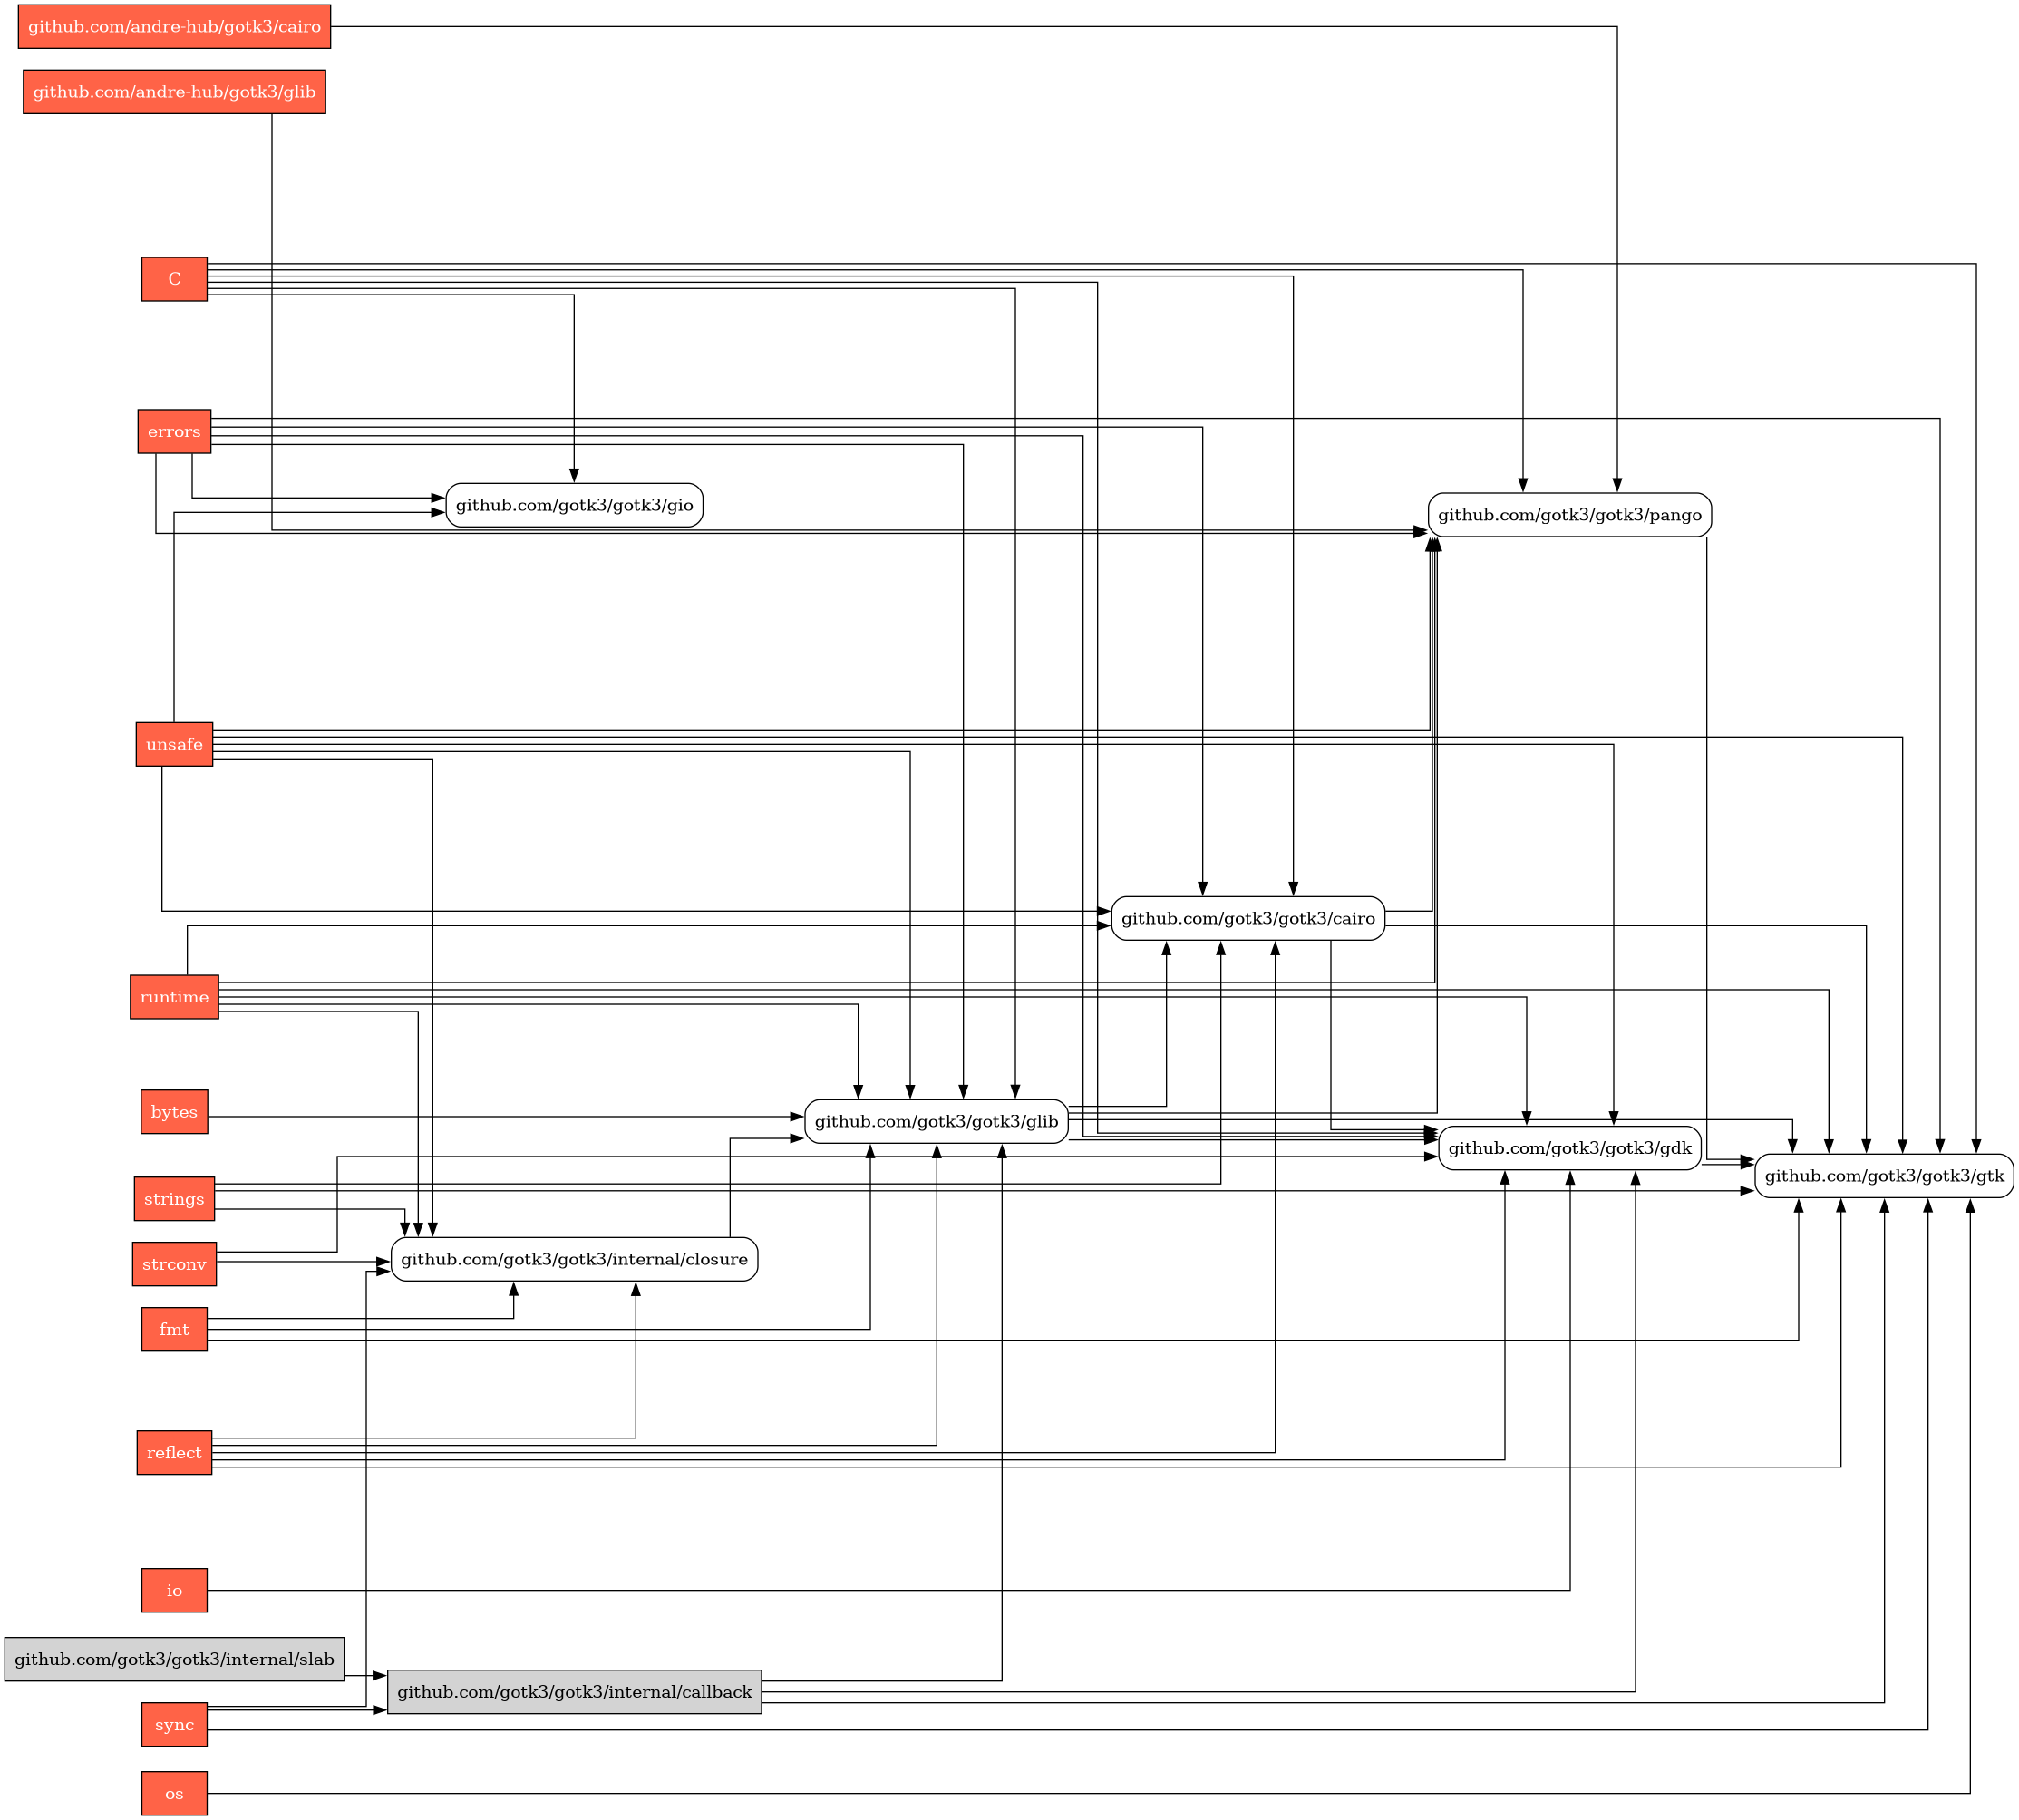
\includegraphics[width=0.7\textwidth]{images/gotk3.png}
        \caption{Grafo do projeto `gotk3`, bindings para GTK3.}
    \end{figure}
    \begin{itemize}
        \item Grafo denso e expansivo, revelando uma arquitetura de "wrappers".
        \item Pacotes Go (`gtk`, `gdk`) espelham a estrutura da biblioteca C subjacente.
    \end{itemize}
\end{frame}

% ---------------------------------------------------------------
\section{Conclusão}
% ---------------------------------------------------------------
\begin{frame}
  \frametitle{Discussão e Conclusão}
  
  \begin{block}{Discussão dos Resultados}
    A ferramenta foi capaz de identificar e visualizar diferentes padrões de arquitetura:
    \begin{itemize}
        \item \textbf{Aplicações:} Padrão "consumidor", onde um nó central integra bibliotecas.
        \item \textbf{Frameworks:} Padrão "hub", com um pacote principal que exporta funcionalidades.
        \item \textbf{Bindings:} Padrão "wrapper", com grafos densos que mapeiam sistemas externos.
    \end{itemize}
  \end{block}
  
  \begin{block}{Conclusão}
      A modelagem com grafos e a ordenação topológica são eficazes para a gestão de dependências em Go, permitindo não apenas a detecção de erros (ciclos), mas também uma profunda análise da arquitetura do software.
  \end{block}
\end{frame}

\begin{frame}
  \frametitle{Trabalhos Futuros}
  
    \begin{itemize}
        \item \textbf{Integração com IDEs:}
        \begin{itemize}
            \item Desenvolver um plugin para editores (e.g., VS Code) para fornecer feedback sobre a criação de ciclos em tempo real.
        \end{itemize}
        \bigskip
        \item \textbf{Análise de "Peso" das Arestas:}
        \begin{itemize}
            \item Estender o modelo para quantificar o nível de acoplamento entre pacotes, destacando dependências críticas.
        \end{itemize}
    \end{itemize}
\end{frame}

% ---------------------------------------------------------------
\begin{frame}
  \frametitle{Referências Bibliográficas}
  \small{
      \begin{thebibliography}{99}
        \bibitem{jergensen2011} Jergensen, N. and Axelsen, J. (2011). \textit{An Analysis of the State of Dependency Hell in the .NET Open Source Ecosystem}. In MLR '11.
        \bibitem{donovan2015go} Donovan, A. A. A. and Kernighan, B. W. (2015). \textit{The Go Programming Language}. Addison-Wesley.
        \bibitem{GoSpec} The Go Authors (2024). \textit{The Go Programming Language Specification}. \url{https://go.dev/ref/spec}.
        \bibitem{clrs} Cormen, T. H. et al. (2009). \textit{Introduction to Algorithms}. The MIT Press, 3rd edition.
        \bibitem{kahn1962} Kahn, A. B. (1962). \textit{Topological sorting of large networks}. Communications of the ACM, 5(11):558–562.
        \bibitem{graphviz} The Graphviz Team (2024). \textit{Graphviz - Graph Visualization Software}. \url{https://graphviz.org/}.
      \end{thebibliography}
  }
\end{frame}

% ---------------------------------------------------------------
\begin{frame}
  \vfill
  \centering
  \huge{\textbf{Obrigado!}}
  \vspace{1cm}
  \Large{Perguntas?}
  \vfill
\end{frame}

\end{document}
